\documentclass{beamer}
\mode<presentation>{
  \usetheme{Boadilla}
  \usefonttheme[onlylarge]{structurebold}
  \usefonttheme[stillsansseriflarge]{serif}
  \setbeamerfont*{frametitle}{size=\normalsize,series=\bfseries}
  % \setbeamertemplate{navigation symbols}{}
  \setbeamercovered{transparent}
}
\usepackage[english]{babel}
\usepackage[latin1]{inputenc}
\usepackage{times}
\usepackage[T1]{fontenc}
\usepackage{amsmath}
\usepackage{amssymb}
\usepackage{esint}
\usepackage{hyperref}
\usepackage{tikz}
\usepackage{xkeyval}
\usepackage{xargs}
\usepackage{xcolor}
\usepackage{verbatim}
\usepackage{listings}
\usepackage{multimedia}
\usepackage{bm}
\usepackage{siunitx}
\usetikzlibrary{
  arrows,
  calc,
  decorations.pathmorphing,
  decorations.pathreplacing,
  decorations.markings,
  fadings,
  positioning,
  shapes,
  arrows.meta
}
\usepgfmodule{oo}

\pgfdeclareradialshading{glow2}{\pgfpoint{0cm}{0cm}}{
  color(0mm)=(white);
  color(2mm)=(white);
  color(8mm)=(black);
  color(10mm)=(black)
}
\pgfdeclareradialshading{glow}{\pgfpoint{0cm}{0cm}}{
  color(0mm)=(white);
  color(5mm)=(white);
  color(9mm)=(black);
  color(10mm)=(black)
}

\begin{tikzfadingfrompicture}[name=glow fading]
  \shade [shading=glow] (0,0) circle (1);
\end{tikzfadingfrompicture}

\begin{tikzfadingfrompicture}[name=glow2 fading]
  \shade [shading=glow2] (0,0) circle (1);
\end{tikzfadingfrompicture}

\mode<handout>{
  \usepackage{pgfpages}
  \pgfpagesuselayout{4 on 1}[a4paper,landscape,border shrink=5mm]
  \setbeamercolor{background canvas}{bg=black!10}
}

\newcommand\pgfmathsinandcos[3]{%
  \pgfmathsetmacro#1{sin(#3)}%
  \pgfmathsetmacro#2{cos(#3)}%
}
\newcommand\LongitudePlane[3][current plane]{%
  \pgfmathsinandcos\sinEl\cosEl{#2} % elevation
  \pgfmathsinandcos\sint\cost{#3} % azimuth
  \tikzset{#1/.estyle={cm={\cost,\sint*\sinEl,0,\cosEl,(0,0)}}}
}
\newcommand\LatitudePlane[3][current plane]{%
  \pgfmathsinandcos\sinEl\cosEl{#2} % elevation
  \pgfmathsinandcos\sint\cost{#3} % latitude
  \pgfmathsetmacro\yshift{\cosEl*\sint}
  \tikzset{#1/.estyle={cm={\cost,0,0,\cost*\sinEl,(0,\yshift)}}} %
}
\newcommand\DrawLongitudeCircle[2][1]{
  \LongitudePlane{\angEl}{#2}
  \tikzset{current plane/.prefix style={scale=#1}}
  % angle of "visibility"
  \pgfmathsetmacro\angVis{atan(sin(#2)*cos(\angEl)/sin(\angEl))} %
  \draw[current plane] (\angVis:1) arc (\angVis:\angVis+180:1);
  \draw[current plane,dashed] (\angVis-180:1) arc (\angVis-180:\angVis:1);
}
\newcommand\DrawLatitudeCircleArrow[2][1]{
  \LatitudePlane{\angEl}{#2}
  \tikzset{current plane/.prefix style={scale=#1}}
  \pgfmathsetmacro\sinVis{sin(#2)/cos(#2)*sin(\angEl)/cos(\angEl)}
  % angle of "visibility"
  \pgfmathsetmacro\angVis{asin(min(1,max(\sinVis,-1)))}
  \draw[current plane,decoration={markings, mark=at position 0.6 with {\arrow{<}}},postaction={decorate},line width=.6mm] (\angVis:1) arc (\angVis:-\angVis-180:1);
  \draw[current plane,dashed,line width=.6mm] (180-\angVis:1) arc (180-\angVis:\angVis:1);
}
\newcommand\DrawLatitudeCircle[2][1]{
  \LatitudePlane{\angEl}{#2}
  \tikzset{current plane/.prefix style={scale=#1}}
  \pgfmathsetmacro\sinVis{sin(#2)/cos(#2)*sin(\angEl)/cos(\angEl)}
  % angle of "visibility"
  \pgfmathsetmacro\angVis{asin(min(1,max(\sinVis,-1)))}
  \draw[current plane] (\angVis:1) arc (\angVis:-\angVis-180:1);
  \draw[current plane,dashed] (180-\angVis:1) arc (180-\angVis:\angVis:1);
}
\newcommand\coil[1]{
  {\rh * cos(\t * pi r)}, {\apart * (2 * #1 + \t) + \rv * sin(\t * pi r)}
}
\makeatletter
\define@key{DrawFromCenter}{style}[{->}]{
  \tikzset{DrawFromCenterPlane/.style={#1}}
}
\define@key{DrawFromCenter}{r}[1]{
  \def\@R{#1}
}
\define@key{DrawFromCenter}{center}[(0, 0)]{
  \def\@Center{#1}
}
\define@key{DrawFromCenter}{theta}[0]{
  \def\@Theta{#1}
}
\define@key{DrawFromCenter}{phi}[0]{
  \def\@Phi{#1}
}
\presetkeys{DrawFromCenter}{style, r, center, theta, phi}{}
\newcommand*\DrawFromCenter[1][]{
  \setkeys{DrawFromCenter}{#1}{
    \pgfmathsinandcos\sint\cost{\@Theta}
    \pgfmathsinandcos\sinp\cosp{\@Phi}
    \pgfmathsinandcos\sinA\cosA{\angEl}
    \pgfmathsetmacro\DX{\@R*\cost*\cosp}
    \pgfmathsetmacro\DY{\@R*(\cost*\sinp*\sinA+\sint*\cosA)}
    \draw[DrawFromCenterPlane] \@Center -- ++(\DX, \DY);
  }
}
\newcommand*\DrawFromCenterText[2][]{
  \setkeys{DrawFromCenter}{#1}{
    \pgfmathsinandcos\sint\cost{\@Theta}
    \pgfmathsinandcos\sinp\cosp{\@Phi}
    \pgfmathsinandcos\sinA\cosA{\angEl}
    \pgfmathsetmacro\DX{\@R*\cost*\cosp}
    \pgfmathsetmacro\DY{\@R*(\cost*\sinp*\sinA+\sint*\cosA)}
    \draw[DrawFromCenterPlane] \@Center -- ++(\DX, \DY) node {#2};
  }
}
\makeatother

% not mandatory, but I though it was better to set it blank
\setbeamertemplate{headline}{}
\def\beamer@entrycode{\vspace{-\headheight}}

\tikzstyle{snakearrow} = [decorate, decoration={pre length=0.2cm,
  post length=0.2cm, snake, amplitude=.4mm,
  segment length=2mm},thick, ->]

%% document-wide tikz options and styles

\tikzset{%
  % >=latex, % option for nice arrows
  inner sep=0pt,%
  outer sep=2pt,%
  mark coordinate/.style={inner sep=0pt,outer sep=0pt,minimum size=3pt,
    fill=black,circle}%
}
\tikzset{
  % Define standard arrow tip
  >=stealth',
  % Define style for boxes
  punkt/.style={
    rectangle,
    rounded corners,
    draw=black, very thick,
    text width=8em,
    minimum height=2.5em,
    text centered},
}

\tikzset{onslide/.code args={<#1>#2}{%
    \only<#1>{\pgfkeysalso{#2}}
    % \pgfkeysalso doesn't change the path
  }}
\tikzset{alt/.code args={<#1>#2#3}{%
    \alt<#1>{\pgfkeysalso{#2}}{\pgfkeysalso{#3}}
    % \pgfkeysalso doesn't change the path
  }}
\tikzset{temporal/.code args={<#1>#2#3#4}{%
    \temporal<#1>{\pgfkeysalso{#2}}{\pgfkeysalso{#3}}{\pgfkeysalso{#4}}
    % \pgfkeysalso doesn't change the path
  }}

\makeatletter
\newbox\@backgroundblock
\newenvironment{backgroundblock}[2]{%
  \global\setbox\@backgroundblock=\vbox\bgroup%
  \unvbox\@backgroundblock%
  \vbox to0pt\bgroup\vskip#2\hbox to0pt\bgroup\hskip#1\relax%
}{\egroup\egroup\egroup}
\addtobeamertemplate{background}{\box\@backgroundblock}{}
\makeatother

% \def\timeleft{15:00->14:55}

\title[EURIQA Brassboard]{A next-generation trapped ion quantum computing system}
\date{June 2, 2022}
\author[Yichao Yu]{Yichao Yu\\
  \vspace{0.5cm}
  {\footnotesize Lei Feng, Liudmila Zhukas, Marko Cetina, Crystal Noel, Debopriyo Biswas,}\\
  {\footnotesize Andrew Risinger, Alexander Kozhanov, Christopher R Monroe}}
\institute[Duke Quantum Center]{Monroe Group/Duke Quantum Center}

\ifpdf
  % Ensure reproducible output
  \pdfinfoomitdate=1
  \pdfsuppressptexinfo=-1
  \pdftrailerid{}
  \hypersetup{
    pdfcreator={},
    pdfproducer={}
  }
\fi

\begin{document}

%% Remarks
% * Improvement compared to the first generation
% * Current status

%% Outline
% * Using Yb ions
% _ * Energy level
% _ * State preparation (time, fidelity)
% _ * State detection (time, fidelity)
% _ * MS gate
% * First generation EURIQA experiment
% _ Results like ..... (Link to DAMOP)
% * Improvements from first generation
% _ * New trap
% _ * Raman system
% _ * Vacuum
% * Status
% _ * Assembly
% _ * Raman beam cross talk
% _ * Trapping and initial characterization

%% Title
% I'm Yichao from the Monroe group at Duke Quantum Center
% and today I'll tell you about our second generation quantum computing experiment.

% Figures
% * (background) lab picture

{
  \usebackgroundtemplate{
    \makebox[\paperwidth][c]{\centering\includegraphics[width=\paperwidth]{imgs/LabPicture_bg.png}}
  }
  \begin{frame}{}
    \titlepage
  \end{frame}
}

% Questions:
% * 355nm power on ions
% * use of 355nm to reduce light shift
% * which transverse mode do we use
% * qubit fidelity
% * main limiting factors
% * breadboard/HOA heating rate
% * what limits gate time? motional mode/laser intrinsic issues
% * Anything else worth mentioning about the oven
% * Reordering graph, what is it showing
% * conversion between pressure and ion reordering rate

%% Yb ions
% In our group, we are building quantum computers using trapped Yb 171 ions.
% As many people here would know, these are good choice for qubits mostly thanks to
% their internal structures. For a start, it got a electronic ground state with
% a J=1/2 and I=1/2 meaning that we have a pair of mF=0 states
% that are insensitive to the B field to the first order.
% This is what has allowed people to achieve a very long coherence time of ~1hr.
% The Yb ion also has a mostly cycling optical transition at 369nm which we can use to
% do fast imaging, state preparation and detection with high fidelity.
% The occational leak into a different electronic D state can be closed with
% a 935nm IR light fairly easily as well.

\begin{frame}{$^{171}\text{Yb}^+$ qubit}
  \begin{center}
    \begin{columns}
      \column{6.5cm}
      \begin{block}{}
        \begin{itemize}
        \item<1-> Long coherence time: $T_2\approx1 \text{hr}$\\
          {\scriptsize Wang, et al., Nat Commun 12, 233 (2021)}\\
          \vspace{1em}
        \item<2-> High fidelity state preparation: $> 99.9\%$ in $\approx 10 \mathrm{\mu s}$
        \item<2-> High speed and high fidelity readout: $> 99.3\%$ in $\approx 100 \mathrm{\mu s}$\\
          \vspace{0.5em}
          {\scriptsize Harty, et al., PRL. 113, 22051, (2014)}
          {\scriptsize Christensen, et al., NPJ Quantum Inf. 6, 35 (2020)}
        \end{itemize}
      \end{block}
      \column{5cm}
      \begin{tikzpicture}
        \begin{scope}[scale=0.8]
          \draw[line width=1] (-0.6, -3) -- node[above right] {$|\!\downarrow\rangle$} (0.6, -3);
          \draw[line width=1] (-2.1, -2.15) -- (-0.9, -2.15);
          \draw[line width=1] (-0.6, -2) --
          node[above right] {$|\!\uparrow\rangle$} (0.6, -2);
          \draw[line width=1] (0.9, -1.85) -- (2.1, -1.85);
          \node[left] at (-2.1, -2.5) {$^2\mathrm{S}_{1/2}$};

          \visible<2->{
            \begin{scope}[shift={(0, 6)}]
              \draw[line width=1] (-0.6, -3) -- (0.6, -3);
              \draw[line width=1] (-2.1, -2.1) -- (-0.9, -2.1);
              \draw[line width=1] (-0.6, -2) -- (0.6, -2);
              \draw[line width=1] (0.9, -1.9) -- (2.1, -1.9);
              \node[left] at (-2.1, -2.5) {$^2\mathrm{P}_{1/2}$};
            \end{scope}

            \draw[snakearrow,line width=1,blue] (0, -2.5) --
            node[right] {$369$ nm} (0, 3.5);
          }
        \end{scope}
      \end{tikzpicture}
    \end{columns}
  \end{center}
\end{frame}

% The ions are trapped in a chain above a surface trap, which give us
% fine control on the axial position of the ions using the surface electrodes.
% For coherent manipulation of these qubit states,
% we use a commercial pulsed laser at 355nm.
% Compared to using CW lasers, these laser systems can provide much higher power,
% allowing us to achieve fast gate operation, and relatively low maintanance,
% which reduces the down time of our experiment.
% Finally, in order to entangle these qubits, we use the momentum kicks
% from our Raman beam to implement a MS gate on the radial mode of
% the shared motional state of the ion chain.

% Figures:
% * Surface trap
% * Paladin

\begin{frame}{$^{171}\text{Yb}^+$ chain and coherent manipulation}
  \begin{center}
    \begin{tikzpicture}
      \node at (3, 2.5) {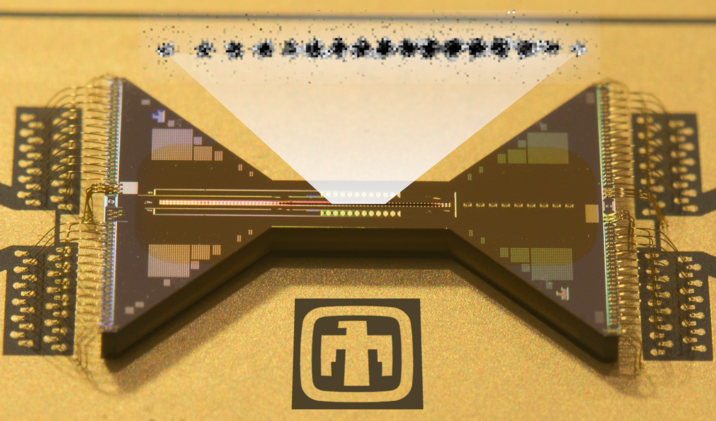
\includegraphics[width=5cm]{imgs/Phoenix_with_ion}};
      \visible<2->{
        \node at (3, -1.5) {\includegraphics[width=5cm]{imgs/Paladin_Breadboard}};
        \begin{scope}[shift={(-3, 0)}]
          \draw[line width=1] (-1.0, -3) -- node[above] {\small $|0, 0\rangle$} (1.0, -3);
          \draw[line width=1] (-1.0, -2) -- node[above] {\small $|1, 0\rangle$} (1.0, -2);
          \draw[line width=1] (-1.5, 2.5) node[left] {$^2\mathrm{P}_{1/2}$} -- (1.5, 2.5);
          \draw[line width=1,dashed] (-1.5, 3) -- (1.5, 3);
          \draw[line width=1] (-1.5, 4) node[left] {$^2\mathrm{P}_{3/2}$} -- (1.5, 4);
          \draw[blue,<->,line width=1] (-0.8, -3) -- node[left] {$355$ nm} (0, 3);
          \draw[blue,<->,line width=1] (0.8, -2) -- (0, 3);

          \draw[<->,dashed,line width=0.5] (0.95, -2) --
          node[right] {$12.6$ GHz} (0.95, -3);
          \draw[<->,dashed,line width=0.5] (1.2, 2.5) --
          node[right] {$33$ THz} (1.2, 3);
          \draw[<->,dashed,line width=0.5] (1.2, 3) --
          node[right] {$66$ THz} (1.2, 4);
        \end{scope}
      }
    \end{tikzpicture}
  \end{center}
\end{frame}

%% First generation system
% Based on these designs, our first generation EURIQA system is able to
% achieve high fidelity single and two qubit operations on 15-24 qubits
% The system can be universally reconfigured/reprogrammed to run
% different kinds of circuits and it's even stable and autonomous enough
% for us to run it almost completely remotely.
% You can hear more about the results from this system,
% and from many of our other experiments in this conference as shown in this list.

% Figures:
% * EURIQA picture

\begin{frame}{$1^{\text{st}}$ generation EURIQA system}
  \begin{center}
    \textbf{E}rror-corrected \textbf{U}niversal \textbf{R}econfigurable
    \textbf{I}on-trap \textbf{Q}uantum \textbf{A}rchetype
    \begin{columns}
      \column{5.2cm}
      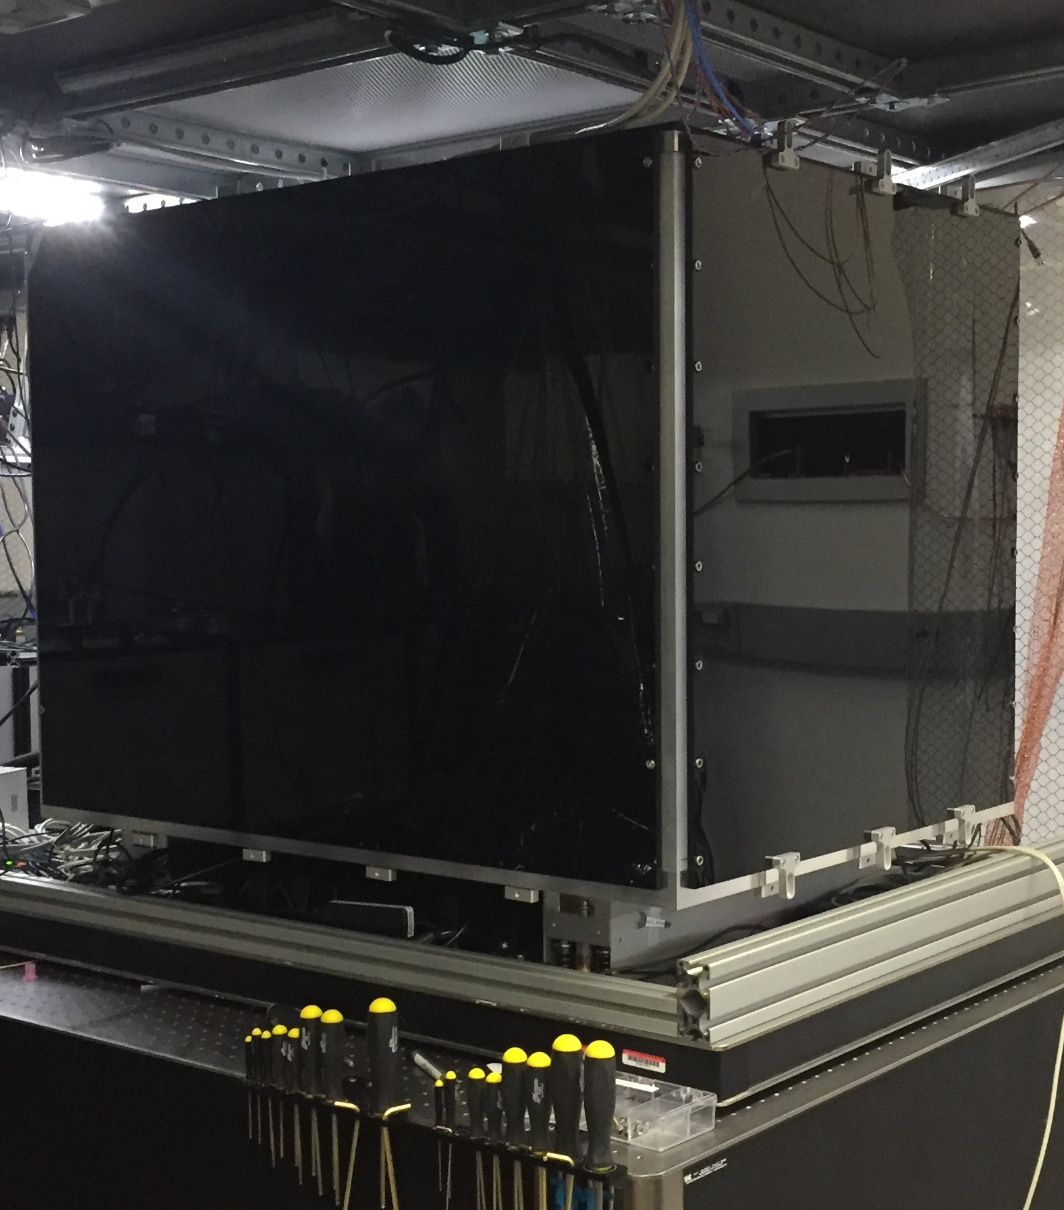
\includegraphics[width=5cm]{imgs/Breadboard_box}
      \column{6.3cm}
      \begin{block}{}
        \begin{itemize}
        \item 15-24 qubits
        \item<2-> High fidelity single and two qubit gates
        \item<3-> Universal reconfigurable
        \item<4-> Remote operations
        \end{itemize}
      \end{block}
      \visible<5->{
        \scriptsize
        \begin{itemize}
        \item E06: Programmable N-body interactions with trapped ion qubits
        \item E06: Implementing Real-Time Logical Qubit Error Detection \&
          Correction on a Trapped Ion Quantum Computer
        \item Q07: Implementation of interactive proofs for quantum advantage
          on an ion-trap quantum computer
        \item U05: Using a trapped ion quantum computer to simulate NMR spectra*
        \end{itemize}
      }
    \end{columns}
  \end{center}
\end{frame}

%% Second generation system
% During the operation of the first system, however, we have identified
% a few limitations of our system that affects the maximum size and fidelity of
% the circuits we run. This is why we are building the second generation EURIQA
% system that is designed to improve on most of these limitations
% based on what we've learnt. You can see an overview of some of the new features here
% and this is what I'm going to focus on for the rest of the talk.

% Figures:
% * Whole system rendering
% * Phoenix
% * Harris
% * Vacuum
% * AOSense

%% TODO: arrow

\begin{frame}{$2^{\text{nd}}$ generation EURIQA system}
  \begin{center}
    \vspace{-0.5cm}
    \begin{tikzpicture}
      \node at (0, 0) {\includegraphics[width=7.5cm]{imgs/Brassboard_render}};
      \node[align=center,font=\tiny] at (-3.8, 3.0)
      {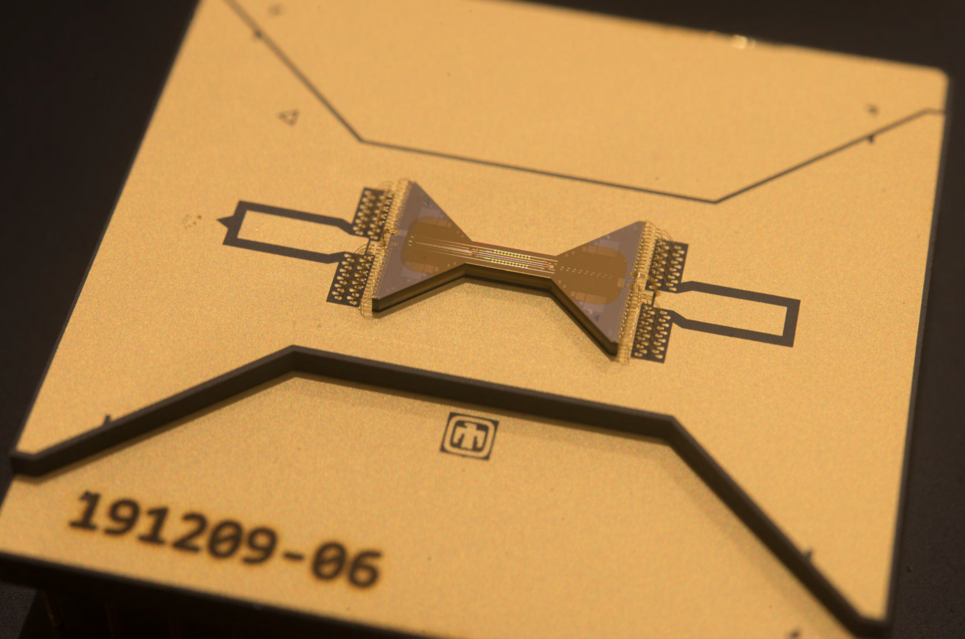
\includegraphics[width=2.3cm]{imgs/Phoenix_zoomout}\\
        Sandia Phoenix trap};
      \node[align=center,font=\tiny] at (-2.7, -3.0)
      {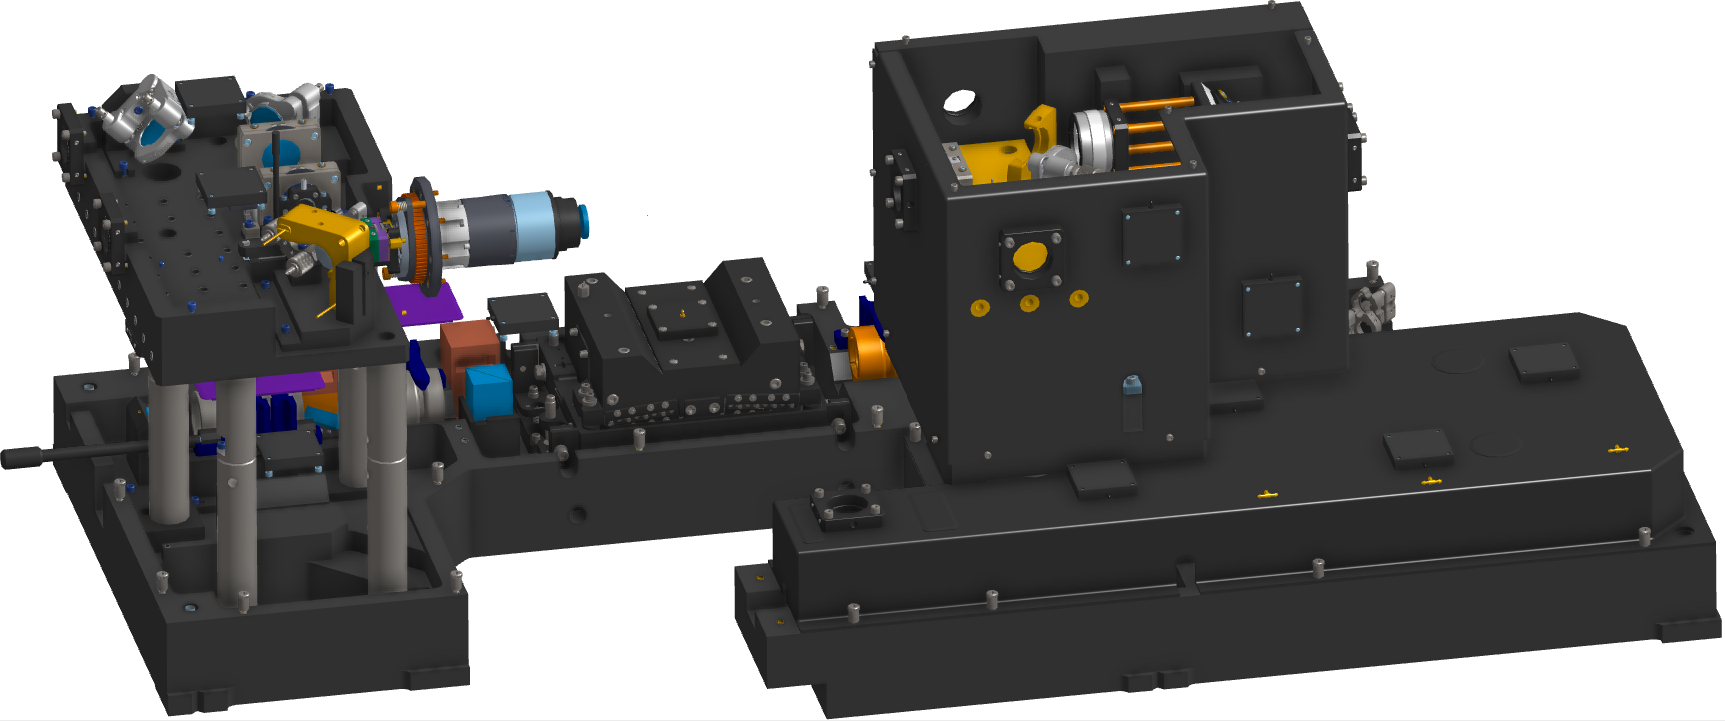
\includegraphics[width=4cm]{imgs/Harris_overview}\\
        L3Harris Raman beam path};
      \node[align=center,font=\tiny] at (3.9, 2.7)
      {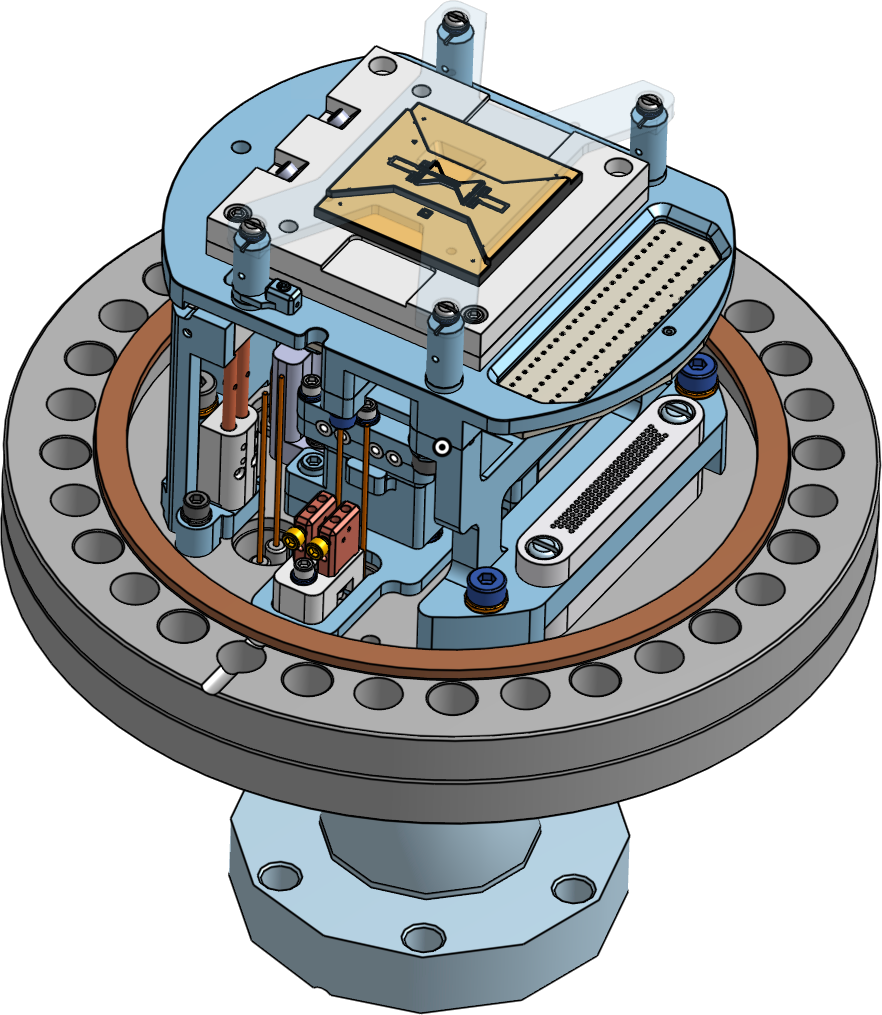
\includegraphics[width=2.6cm]{imgs/Vacuum_stack}\\
        Improved vacuum system};
      \node[align=center,font=\tiny] at (3.9, -2.5)
      {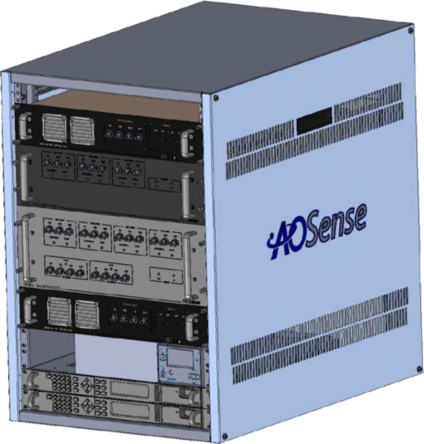
\includegraphics[width=2.4cm]{imgs/AOSense_external}\\
        CW lasers};
    \end{tikzpicture}
  \end{center}
\end{frame}

%% Phoenix trap
% One of the main issues that limits the gate fidelity and ion numbers
% in the 1st generation experiment is the heating of ions from surface
% electric field noise and that's indeed one of the main focus of the design.

% We use the Pheonix trap which is a new generation of the surface trap
% from the Snadia National Lab. It has better wall metallization,
% which should shield and reduce the field noise as well as reducing
% charging and photovoltaic effect caused by stray laser beams.
% It also comes with segmented outter electrodes which give us better control
% on the ion chain for compensating micromotion across the whole chain.
% All of these contributes to a lower heating rate when we run our gates
% on the ion chain. (show number)

% Additionally, the loading rate of the trap is also improved thanks to a larger
% loading slot and a simpler trap geometry
% allowing shuttling of multiple ions simutaniously.

% Figures:
% * Phoenix
% * Outer electrodes
% * Loading slot

\begin{frame}{$2^{\text{nd}}$ gen EURIQA: Pheonix trap}
  \begin{center}
    \begin{tikzpicture}
      \node[text width=6.5cm] at (-3, 2) {
        \begin{itemize}
        \item Better metallization
          \begin{itemize}
          \item Reducing noise
          \item Less charging/photovoltaic effect
          \end{itemize}
          30 qunta/s @ 3 MHz heating rate
        \item Segmented outter electrodes
        \item Better and faster ion loading
        \end{itemize}
      };
      \node at (3, 2) {\includegraphics[width=4.8cm]{imgs/Phoenix}};
      \node at (3.5, -2) {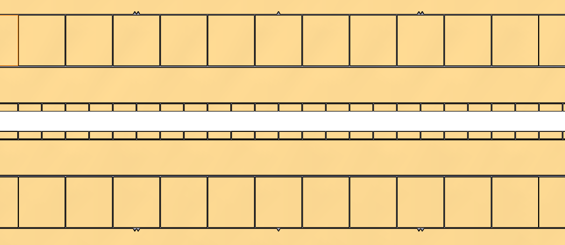
\includegraphics[width=4.8cm]{imgs/Phoenix_quantum}};
      \node at (-2.5, -2) {\includegraphics[width=4.3cm]{imgs/Phoenix_Loading_SEM}};
    \end{tikzpicture}
  \end{center}
\end{frame}

%% Raman geometry
% Another main change we made to improve our gate fidelity is the Raman beam geometry.
% Compared to the 1st generation experiment, which send one of the Raman beams
% perpendicular to the trap surface, we send both of our Raman beams parallel
% to the trap. This means that the motional mode we use is also parallel to the surface,
% and has minimum coupling to the dominant E field noise.
% The momentum transfer from the Raman transition is also faster,
% allowing faster gate operations.
% Not having to send our Raman beam through the trap should also reduces
% the amount of field noise induced by the laser.

\begin{frame}{$2^{\text{nd}}$ gen EURIQA: Raman geometry}
  \begin{center}
    \begin{tikzpicture}
      \begin{scope}[shift={(-3, 0)}]
        \node at (0, 2) {\includegraphics[width=4.6cm]{imgs/Breadboard_Raman.png}};

        \draw[->,blue!80!black,line width=1] (-1.9, -2.5) --
        node[below] {$k_g$} (-0.1, -2.5);
        \draw[->,blue!80!black,line width=1] (0, -0.6) --
        node[right] {$k_i$} (0, -2.4);
        \draw[->,green!70!black,line width=1] (-1.9, -2.4) --
        node[above,sloped] {$\Delta k$} (-0.1, -0.6);

        \draw[->,red!60!black,line width=0.7] (2.1, -3.1) --
        node[below,sloped] {E field noise} (2.1, -0.9);
      \end{scope}

      \begin{scope}[shift={(3, 0)}]
        \node at (0, 2) {\includegraphics[width=4.6cm]{imgs/Brassboard_Raman.png}};

        \draw[->,blue!80!black,line width=1] (-1.9, -2.5) --
        node[below] {$k_g$} (-0.1, -2.5);
        \draw[->,blue!80!black,line width=1] (1.9, -2.5) --
        node[below] {$k_i$} (0.1, -2.5);
        \draw[->,green!70!black,line width=1] (-1.9, -2.3) --
        node[above,sloped] {$\Delta k$} (1.9, -2.3);

        \draw[->,red!60!black,line width=0.7] (2.1, -3.1) --
        node[below,sloped] {E field noise} (2.1, -0.9);
      \end{scope}
    \end{tikzpicture}
  \end{center}
\end{frame}

%% New oven
% In the 1st gen experiment, we demostrated an improvment in circuit depth
% by sympathetically cooling the ion chain using Yb 172 icon.
% To accommodate this better, we've changed our atomic source to one with higher
% Yb 172 abundance. As you can see in this theoretical plot,
% we can selectively load either an 171 or 172 ion with more than 90% probability
% by changin the frequency of our ionization laser.
% This will help us construct the chain with the composition we want
% more deterministically.

% Figures:
% * Isotope selection plot

\begin{frame}{$2^{\text{nd}}$ gen EURIQA: New Yb atom source}
  \begin{center}
    \begin{columns}
      \column{6.3cm}
      \begin{itemize}
      \item Sympathetic cooling with $^{172}\mathrm{Yb}^+$\\
        {\scriptsize Cetina, et al., PRX Quantum 3, 010334 (2022)}\\
        \vspace{1em}
      \item New Yb source to enhance loading of $^{172}\mathrm{Yb}^+$
      \end{itemize}
      \column{5.1cm}
      \includegraphics[width=5cm]{imgs/Loading_Frequency.png}
    \end{columns}
  \end{center}
\end{frame}

%% Construction
% As part of the system upgrade and construction, we've also designed
% and implemented some technical improvements that should help with
% the general operation of the system.
% This includes a better vacuum system built using vacuum-fired low hydrogen components
% This should reduce the hydrogen pressure in our chamber and therefore
% improve upon the 4-5min time between collisions measured in our first gen system.
% We have pumped down our chamber and we are currently measuring
% a 9e-12 Torr pressure in our system.
% We'll need to check the collision rate with the ions after we trap a chain of them.

% Figures:
% * Vacuum drawing
% * Reordering plot

\begin{frame}{$2^{\text{nd}}$ gen EURIQA: Improved vacuum}
  \begin{center}
    \begin{columns}
      \column{6.3cm}
      \begin{itemize}
      \item Vacuum fired components
      \item Reduce ion-chain reordering rate
      \end{itemize}
      \begin{center}
        \includegraphics[width=5cm]{imgs/Reorder_rate.png}\\
        {\footnotesize 15-ion chain reorders every 4-5 min}\\
        {\footnotesize in $1^{\text{st}}$ gen EURIQA system.}\\
        {\scriptsize Cetina, et al.}
      \end{center}
      \column{5.1cm}
      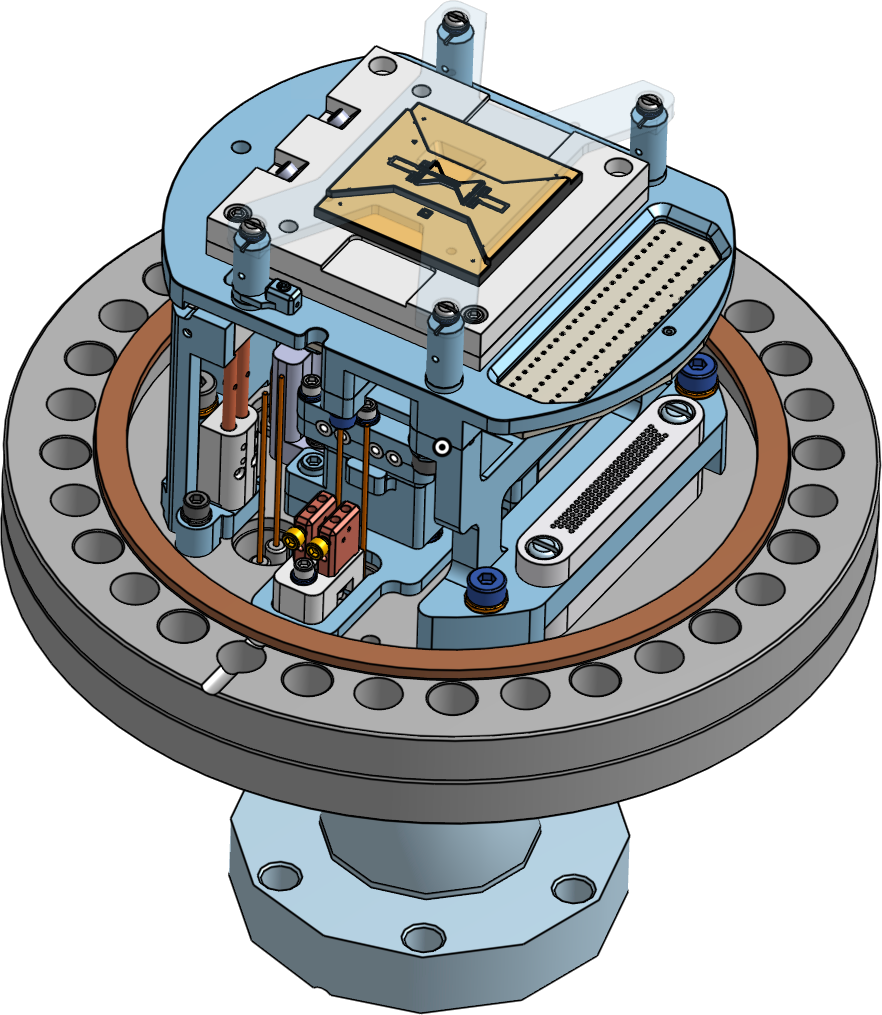
\includegraphics[width=5cm]{imgs/Vacuum_stack.png}
    \end{columns}
  \end{center}
\end{frame}

% We also have a specially build Raman deliverying beam path built by L3Harris
% that is more stable and purged with clean nitrogen to reduce UV burn on the optics.
% This Raman delivery system was just aligned and commissioned thanks to people from
% L3Harris a few months ago as you can see in this picture.
% We have optically characterized the shape of our global and individual
% addressing Raman beams which shows promising performance especially
% in terms of the cross talk to the neighboring ions.

% Figures:
% * Harris picture/drawing
% * Beam images

% TODO: mark spacing on individual

\begin{frame}{$2^{\text{nd}}$ gen EURIQA: Raman beam path}
  \begin{center}
    \begin{tikzpicture}
      \node at (0, 0) {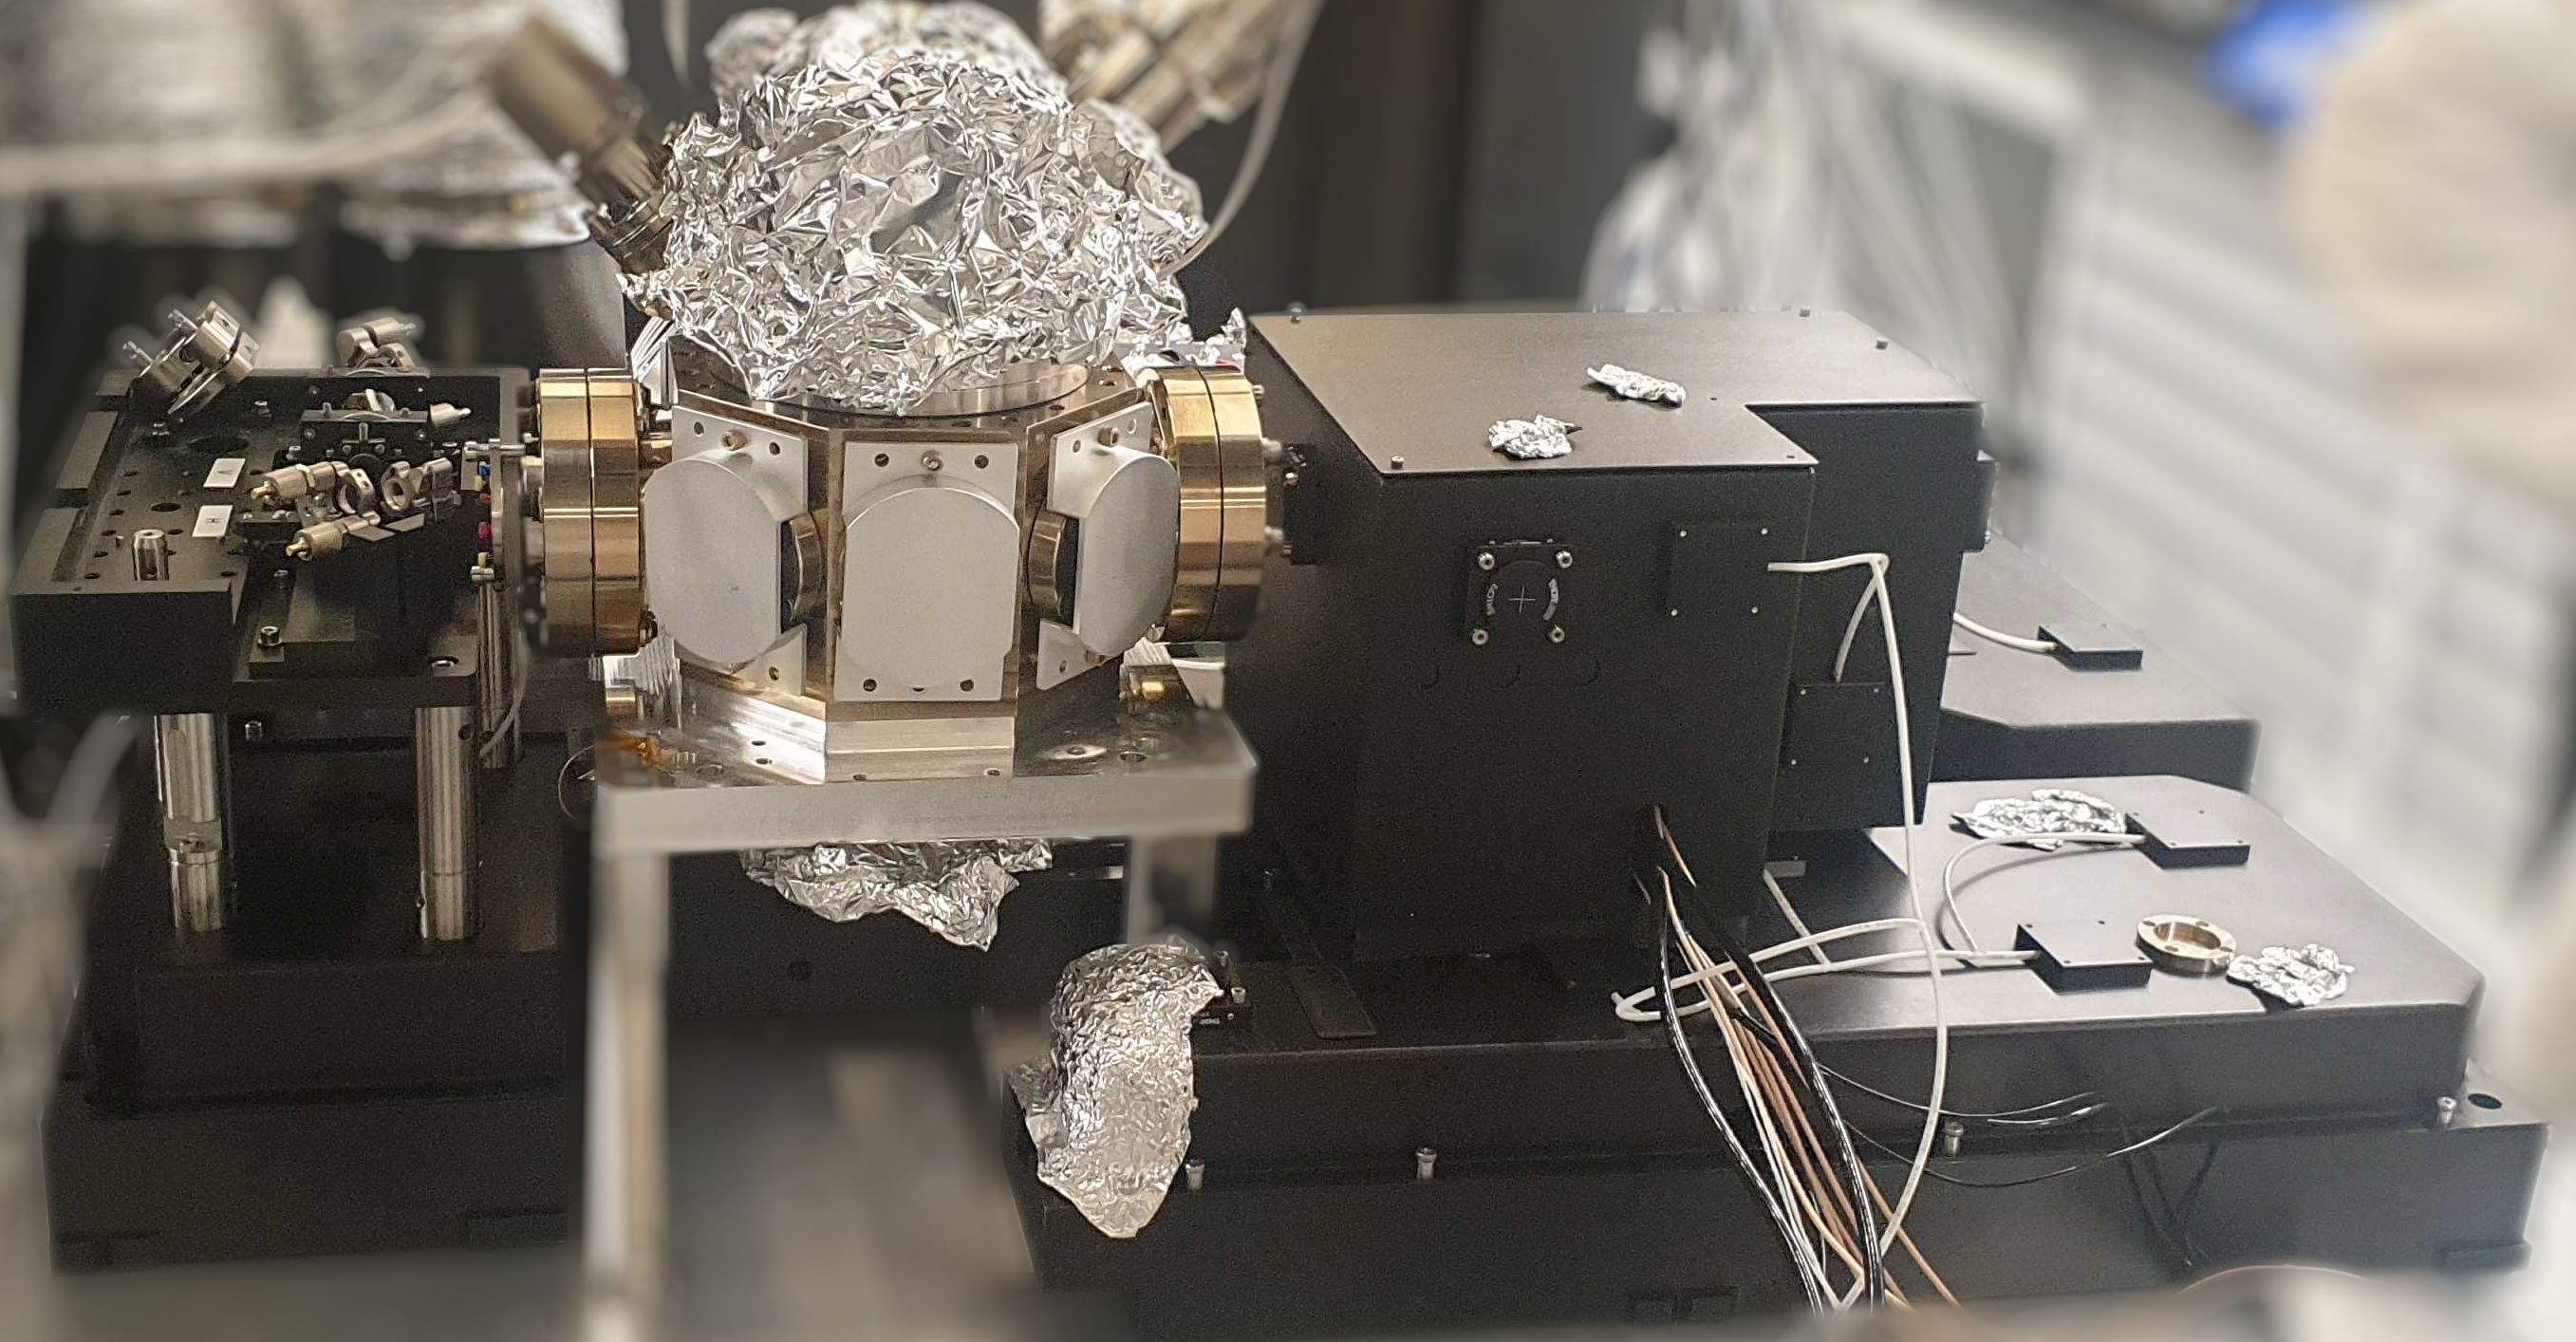
\includegraphics[width=10cm]{imgs/Harris_optics.png}};
      \fill[white,opacity=0.8] (-5.05, -3.2) rectangle (5.05, 3.2);
      \node[align=center] at (0, 2) {\large Global addressing Raman beam\\
        
\includegraphics[height=1cm]{imgs/Global_beam.png}};
      \node[align=center] at (0, -2) {\large Individual addressing Raman beam\\
        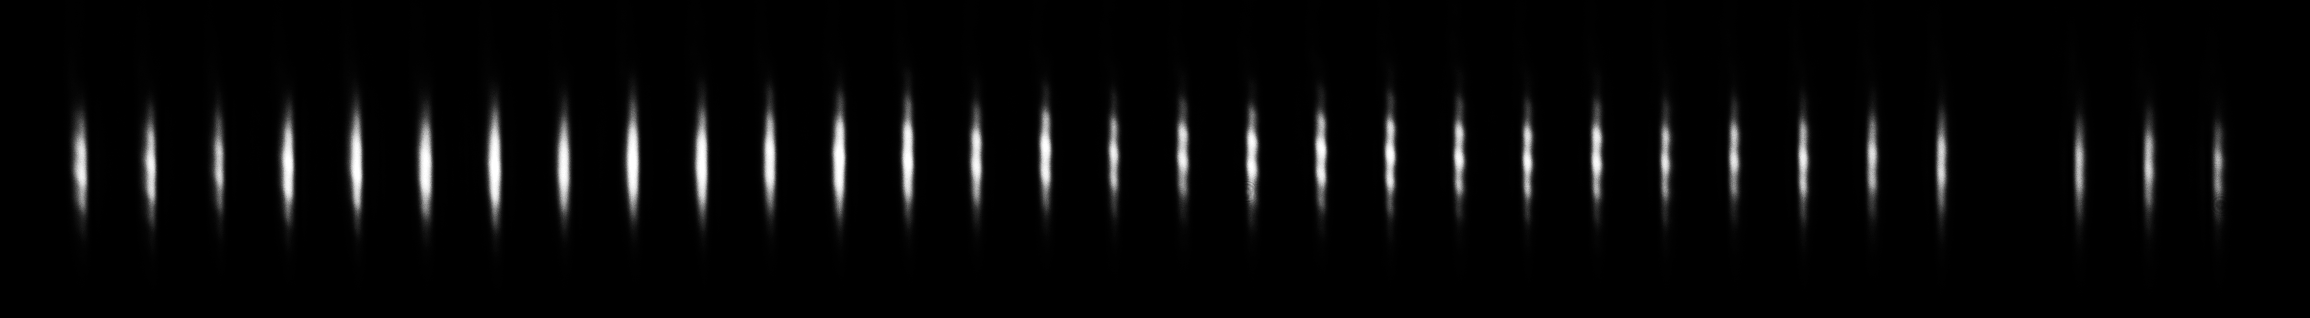
\includegraphics[height=1.5cm]{imgs/Individual_beam.png}};
    \end{tikzpicture}
  \end{center}
\end{frame}

% The CW lasers for cooling and trapping of the ions has also been upgraded
% to a system built by AOSense for us. The whole beam path is built
% on a single piece of aluminum base board and with my hand there for scale,
% you can see that the optics and beam path are quite compact.
% These design features should improve the stability of our beam path.
% We've already aligned and commissioned most of the beam path
% and we'll learn more about their stability as we operate the system.

% Figures:
% * AOSense internal picture
% * AOSense alignment picture

\begin{frame}{$2^{\text{nd}}$ gen EURIQA: CW lasers}
  \begin{center}
    \begin{tikzpicture}
      \node at (-2.2, -1) {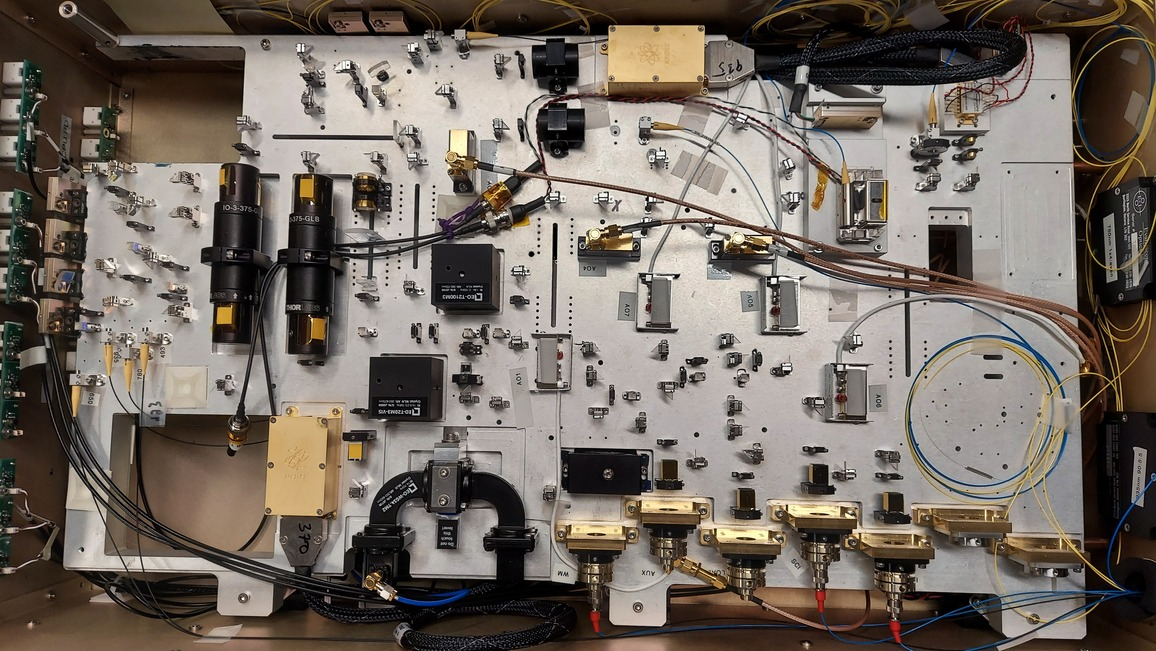
\includegraphics[width=7.5cm]{imgs/AOSense_internal.jpg}};
      \node at (4, 0) {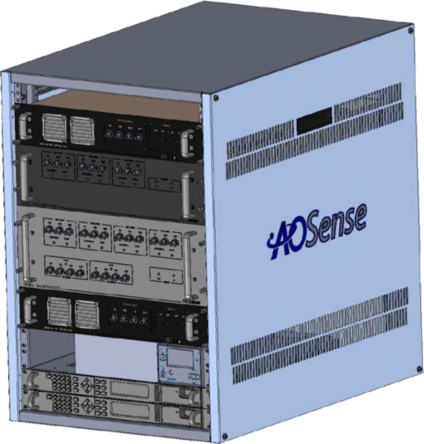
\includegraphics[width=4cm]{imgs/AOSense_external.png}};
      \node[align=left] at (-2.2, 2.5) {Rack mounted miniaturized beam path\\
        for 369, 399, 780 and 935 nm.};
      \node at (0, 0) {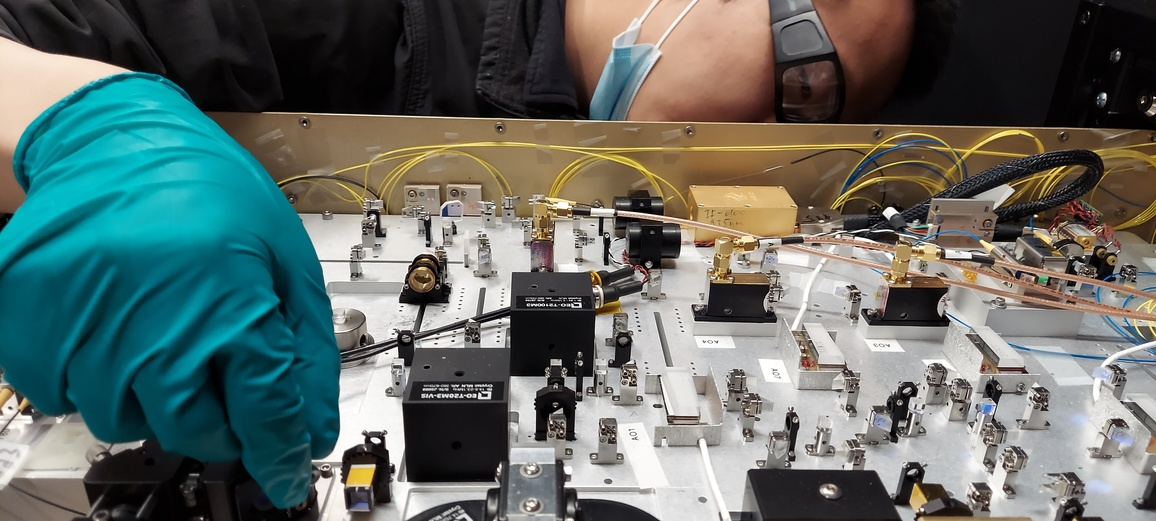
\includegraphics[width=11.5cm]{imgs/AOSense_align.jpg}};
    \end{tikzpicture}
  \end{center}
\end{frame}

%% Current status
% The system, with all of the improved design in place, is shown in this photo.
% Here you can see our vacuum chamber, with the delivery beam path for the CW lasers
% mounted on it, and the Raman beam path from L3Harris surrounding it.
% We have trapped Yb 171 ions in the chamber as of two weeks ago
% as you can see in this picture.
% We've also started characterizing our system
% as well as the optimization for various parameters,
% moving towards operating quantum gates in our system.
% Here I'll leave you with a video showing our first measurement of
% the secular frequency using parametric heating.

% Figures:
% * Lab picture
% * Ion picture
% * Ion heating video

\begin{frame}{$2^{\text{nd}}$ gen EURIQA: status and first ion}
  \begin{center}
    \begin{tikzpicture}
      \node at (0, 0) {\includegraphics[width=10.5cm]{imgs/LabPicture.png}};
    \end{tikzpicture}
  \end{center}
\end{frame}

\begin{frame}{}
\end{frame}

\end{document}
